\documentclass[10pt,a4paper]{article}

% content/resources/templates/preamble.tex
\usepackage[margin=0.6in]{geometry}
\author{Milav Dabgar}
\usepackage{amsmath,amssymb,amsthm}
\usepackage{booktabs}
\usepackage{multirow}
\usepackage{xcolor}
\usepackage{tcolorbox}
\tcbuselibrary{breakable,skins}
\usepackage[colorlinks=true,linkcolor=blue]{hyperref}
\usepackage{titlesec}
\usepackage{enumitem}
\usepackage{tikz}
\usepackage{pgfplots}
\usepackage{circuitikz}
\usepackage[version=4]{mhchem}
\usepackage{longtable}
\usepackage{array}
\usepackage{float}
\usepackage{caption}
\usepackage{listings}

\lstset{
  basicstyle=\small\ttfamily,
  breaklines=true,
  breakatwhitespace=false,
  postbreak=\mbox{\textcolor{red}{$\hookrightarrow$}\space},
  float=false,
  numbers=left,
  numberstyle=\tiny\color{gray},
  numbersep=10pt,
  xleftmargin=2em,
  keywordstyle=\color{blue},
  commentstyle=\color{green!60!black},
  stringstyle=\color{purple},
  backgroundcolor=\color{gray!5},
  showstringspaces=false,
  tabsize=2,
  captionpos=b,
  keepspaces=true,
  columns=flexible
}

\pgfplotsset{compat=1.18}
\usetikzlibrary{shapes,arrows,positioning,calc,patterns,decorations.pathmorphing,decorations.markings,arrows.meta}

% Color scheme
\definecolor{headcolor}{RGB}{0,102,204}
\definecolor{keycolor}{RGB}{220,20,60}
\definecolor{solutioncolor}{RGB}{34,139,34}
\definecolor{mnemoniccolor}{RGB}{148,0,211}
\definecolor{codecolor}{RGB}{0,0,100}

% Spacing
\setlength{\parskip}{3pt}
\setlist[itemize]{nosep}
\setlist[enumerate]{nosep}

% Title formatting
\titleformat{\section}{\Large\bfseries\color{headcolor}}{\thesection}{1em}{}
\titleformat{\subsection}{\large\bfseries\color{headcolor}}{\thesubsection}{1em}{}

% Pandoc tightlist compatibility
\providecommand{\tightlist}{%
  \setlength{\itemsep}{0pt}\setlength{\parskip}{0pt}}

% Pandoc longtable compatibility
\newcounter{none}
\def\thenone{}


% content/resources/templates/english-boxes.tex
% This file is currently empty - it exists to maintain consistency with the import structure.
% Add custom environments here if needed in the future.


\begin{document}

\subsection{Question 1(a) {[}3 marks{]}}\label{question-1a-3-marks}

\textbf{Choose the correct option: (Any Three)}

\begin{enumerate}
\def\labelenumi{\arabic{enumi}.}
\item
\begin{solutionbox}
  SMCR Model of Communication was created by \_\_. \textbf{Answer}: C.
  David Berlo
\end{solutionbox}
\item
\begin{solutionbox}
  \_\_\_\_\_ is NOT a part of verbal communication. \textbf{Answer}: B.
  Gesture
\end{solutionbox}
\item
  Factors that influence communication negatively are called \_\_\_\_\_
\begin{solutionbox}
  to effective communication. \textbf{Answer}: A. Barriers
\end{solutionbox}
\item
  The response to a sender's message is called \_\_\_\_.
\begin{solutionbox}
  \textbf{Answer}: D. Feedback
\end{solutionbox}
\end{enumerate}

\subsection{Question 1(b) {[}4 marks{]}}\label{question-1b-4-marks}

\textbf{Answer the following questions: (Any Four)}

\begin{enumerate}
\def\labelenumi{\arabic{enumi}.}
\item
  \textbf{How can you explain the term `communication'?}

\begin{solutionbox}
  \textbf{Answer}: Communication is the process of exchanging
  information, ideas, and feelings between individuals through a common
  system of symbols, signs, or behaviors. It involves a sender
  transmitting a message through a channel to a receiver who provides
  feedback.
\end{solutionbox}
\item
  \textbf{What can you infer from the term `encoding'?}

\begin{solutionbox}
  \textbf{Answer}: Encoding is the process of converting thoughts and
  ideas into symbols, words, or gestures that the receiver can
  understand. It's how the sender transforms the message into a suitable
  format before transmission through the selected communication channel.
\end{solutionbox}
\item
  \textbf{How will you contrast `verbal communication' and `non-verbal
  communication'?}

\begin{solutionbox}
  \textbf{Answer}:

  \textbf{Table: Verbal vs.~Non-verbal Communication}

  {\def\LTcaptype{none} % do not increment counter
  \begin{longtable}[]{@{}
    >{\raggedright\arraybackslash}p{(\linewidth - 2\tabcolsep) * \real{0.4468}}
    >{\raggedright\arraybackslash}p{(\linewidth - 2\tabcolsep) * \real{0.5532}}@{}}
  \toprule\noalign{}
  \begin{minipage}[b]{\linewidth}\raggedright
  Verbal Communication
  \end{minipage} & \begin{minipage}[b]{\linewidth}\raggedright
  Non-verbal Communication
  \end{minipage} \\
  \midrule\noalign{}
  \endhead
  \bottomrule\noalign{}
  \endlastfoot
  Uses words (spoken or written) & Uses body language, gestures,
  expressions \\
  Can be direct and explicit & Often unconscious and implicit \\
  Limited by language barriers & Transcends language barriers \\
  Primarily conveys information & Primarily conveys emotions and
  attitudes \\
  \end{longtable}
  }
\end{solutionbox}
\item
  \textbf{How would you summarise the term `paralanguage'?}

\begin{solutionbox}
  \textbf{Answer}: Paralanguage refers to how we say things rather than
  what we say. It includes voice qualities (pitch, tone, volume), vocal
  characterizers (laughing, crying), vocal qualifiers (intensity,
  rhythm), and vocal segregates (fillers like ``um,'' ``ah''). These
  elements add emotional context to verbal communication.
\end{solutionbox}
\item
  \textbf{If a listener does not know/understand a speaker's language,
  what kind of barrier will it be called?}

\begin{solutionbox}
  \textbf{Answer}: This is a semantic barrier or language barrier. It
  occurs when the sender and receiver use different languages,
  specialized terminology, or jargon that prevents effective
  understanding of the message's intended meaning.
\end{solutionbox}
\end{enumerate}

\subsection{Question 1(c) {[}7 marks{]}}\label{question-1c-7-marks}

\textbf{Answer the following questions: (Any Seven)}

\begin{enumerate}
\def\labelenumi{\arabic{enumi}.}
\item
  \textbf{What must the horse find `queer'?}

\begin{solutionbox}
  \textbf{Answer}: In ``Stopping by Woods on a Snowy Evening,'' the
  horse finds it strange (queer) that the speaker has stopped ``without
  a farmhouse near'' in the dark woods. The horse is confused by the
  unscheduled stop in an uninhabited area, especially during a snowy
  evening.
\end{solutionbox}
\item
  \textbf{``He gives his harness bells a shake'' -- Who is `he'?}

\begin{solutionbox}
  \textbf{Answer}: `He' refers to the horse in the poem. The horse
  shakes its harness bells as if questioning why they've stopped in the
  middle of nowhere, reminding the speaker of their responsibilities and
  journey ahead.
\end{solutionbox}
\item
  \textbf{What does Tagore suggest through the phrase ``mind is without
  fear''?}

\begin{solutionbox}
  \textbf{Answer}: Through the phrase ``mind is without fear,'' Tagore
  suggests a society where people can think and express themselves
  freely without intimidation or oppression. He envisions citizens who
  aren't afraid to voice their opinions or embrace new ideas due to
  political, social, or religious pressure.
\end{solutionbox}
\item
  \textbf{Whom does Tagore address as `my Father'?}

\begin{solutionbox}
  \textbf{Answer}: Tagore addresses God as `my Father' in the poem
  ``Where the Mind is Without Fear.'' This spiritual invocation shows
  Tagore seeking divine help to achieve his vision of a free,
  enlightened nation where reason and truth prevail.
\end{solutionbox}
\item
  \textbf{What was the appointment made between Bob and Jimmy before
  twenty years?}

\begin{solutionbox}
  \textbf{Answer}: Bob and Jimmy had made an appointment to meet at the
  same spot (outside what was Big Joe Brady's restaurant) exactly twenty
  years later at 10 PM, regardless of where life took them. This
  agreement was made over their last dinner together before parting
  ways.
\end{solutionbox}
\item
  \textbf{Why was Bob under arrest?}

\begin{solutionbox}
  \textbf{Answer}: Bob was under arrest because he was a wanted criminal
  from Chicago. During their twenty years apart, while Jimmy had become
  a policeman, Bob had chosen a life of crime and had become a notorious
  criminal with a wanted status, which Jimmy had discovered during his
  police duty.
\end{solutionbox}
\item
  \textbf{What examples of nature can you find to justify `The Leopard'
  as a nature-centric prose?}

\begin{solutionbox}
  \textbf{Answer}: ``The Leopard'' contains numerous nature elements:
  the mountain stream, forktail bird, ravine ecosystem, the leopard
  itself, jungle sounds, seasonal changes, and descriptions of natural
  habitats. The author's detailed observations of flora and fauna and
  their interdependence create a rich nature-centric narrative.
\end{solutionbox}
\item
  \textbf{Why were the shikaris roaming in the forest?}

\begin{solutionbox}
  \textbf{Answer}: The shikaris (hunters) were roaming in the forest to
  hunt and kill the leopard and other wild animals. This represents the
  human threat to wildlife that the author disapproves of, highlighting
  the conflict between human encroachment and wildlife preservation.
\end{solutionbox}
\end{enumerate}

\subsection{OR}\label{or}

\textbf{Answer the following questions: (Any Seven)}

\begin{enumerate}
\def\labelenumi{\arabic{enumi}.}
\item
  \textbf{Which season is described in `Stopping by Woods'?}

\begin{solutionbox}
  \textbf{Answer}: Winter season is described in ``Stopping by Woods on
  a Snowy Evening.'' This is evident from descriptions of snowfall
  (``woods fill up with snow''), the ``darkest evening of the year''
  suggesting winter solstice, and the frozen lake mentioned in the poem.
\end{solutionbox}
\item
  \textbf{Which promises does the poet talk about in `Stopping by Woods
  on a Snowy Evening'?}

\begin{solutionbox}
  \textbf{Answer}: The poet doesn't specify what promises he refers to
  in the line ``And miles to go before I sleep.'' These likely represent
  social obligations, responsibilities, and commitments that demand his
  attention. The repeated line emphasizes both literal journey distance
  and figurative life commitments.
\end{solutionbox}
\item
  \textbf{What does the poet mean by ``knowledge is free''?}

\begin{solutionbox}
  \textbf{Answer}: By ``knowledge is free,'' Tagore envisions a society
  where education and information are accessible to everyone regardless
  of social status, caste, gender, or economic condition. He dreams of
  learning without boundaries, where ideas flow freely without
  restrictive traditions or prejudices.
\end{solutionbox}
\item
  \textbf{What is meant by ``narrow domestic walls''?}

\begin{solutionbox}
  \textbf{Answer}: ``Narrow domestic walls'' refers to artificial
  divisions based on religion, caste, class, language, and region that
  separate people within a country. Tagore criticizes these artificial
  barriers that fragment society and hinder national unity and human
  connection.
\end{solutionbox}
\item
  \textbf{How did Bob realise that the cop was not Jimmy?}

\begin{solutionbox}
  \textbf{Answer}: Bob realized the cop wasn't Jimmy when the
  plainclothes officer (the real policeman who arrested him) mentioned
  that Jimmy had sent him. Additionally, the plainclothes officer
  matched Jimmy's description of his friend, revealing the uniformed cop
  had been Jimmy in disguise who couldn't arrest his friend himself.
\end{solutionbox}
\item
  \textbf{What does the phrase `guardian of peace' mean?}

\begin{solutionbox}
  \textbf{Answer}: The phrase ``guardian of peace'' in ``After Twenty
  Years'' refers to Jimmy Wells' role as a police officer. It highlights
  his duty to uphold law and order, protect citizens, and maintain
  social peace and safety, which ultimately conflicts with his personal
  loyalty to his friend Bob.
\end{solutionbox}
\item
  \textbf{What was the author's attitude towards man in `The Leopard'?}

\begin{solutionbox}
  \textbf{Answer}: In ``The Leopard,'' the author held a critical
  attitude toward humans who disturbed or harmed wildlife. He
  disapproved of hunters (shikaris), expressed concern about human
  encroachment on natural habitats, and preferred animals' company over
  humans'. He valued people who respected nature's balance.
\end{solutionbox}
\item
  \textbf{How was the ravine?}

\begin{solutionbox}
  \textbf{Answer}: The ravine in ``The Leopard'' was described as a
  deep, secluded valley with a stream running through it. It featured
  dense vegetation, rocks, and served as a natural habitat for various
  wildlife including the leopard and forktail. The author portrayed it
  as a peaceful, untouched sanctuary away from human interference.
\end{solutionbox}
\end{enumerate}

\subsection{Question 2(a) {[}3 marks{]}}\label{question-2a-3-marks}

\textbf{Identify the sentence pattern: (Any Three)}

\begin{enumerate}
\def\labelenumi{\arabic{enumi}.}
\item
\begin{solutionbox}
  Sumit / is / happy. \textbf{Answer}: Subject + Verb + Complement (SVC)
\end{solutionbox}
\item
\begin{solutionbox}
  The monk / opened / his eyes. \textbf{Answer}: Subject + Verb + Object
  (SVO)
\end{solutionbox}
\item
\begin{solutionbox}
  I / like / painting. \textbf{Answer}: Subject + Verb + Object (SVO)
\end{solutionbox}
\item
\begin{solutionbox}
  Meena / sang / beautifully. \textbf{Answer}: Subject + Verb + Adverb
  (SVA)
\end{solutionbox}
\end{enumerate}

\subsection{Question 2(b) {[}4 marks{]}}\label{question-2b-4-marks}

\textbf{Fill in the blanks by using the appropriate Modal Auxiliary:
(Any Four)}

\begin{enumerate}
\def\labelenumi{\arabic{enumi}.}
\item
  Shyam \textbf{has to} pay his college fees by tomorrow. (has to,
  could, may)
\item
  We \textbf{must} respect the national flag. (can, must, may)
\item
  I \textbf{would} prefer tea to coffee. (might, must, would)
\item
  \textbf{May} you live long! (Must, May, Should)
\item
  You \textbf{should} not waste your father's money. (may, should,
  might)
\end{enumerate}

\subsection{Question 2(c) {[}7 marks{]}}\label{question-2c-7-marks}

\textbf{Do as directed: (Any Seven)}

\begin{enumerate}
\def\labelenumi{\arabic{enumi}.}
\item
  Vimal is a \textbf{sincere} student. (Identify `adjective')
\item
  \textbf{Manish} was ill yesterday, so \textbf{he} did not attend
  classes. (Identify `pronoun')
\item
  These \textbf{fruits} are fresh. (Identify `noun')
\item
  Asmita sings \textbf{melodiously}. (Identify `adverb')
\item
  Kandarp will undergo a surgery \textbf{in} the next month. (Identify
  `preposition')
\item
  Identify the sentence in present continuous tense -- It rains. / It
  rained. / \textbf{It is raining}.
\item
  The past participle tense form of `catch' is \textbf{caught}.
  (catched, caught, catch)
\item
  The word `will' is placed before a verb in case of a sentence of
  \textbf{Simple Future} tense. (Simple Past, Simple Present, Simple
  Future)
\end{enumerate}

\subsection{OR}\label{or-1}

\subsection{Question 2(a) {[}3 marks{]}}\label{question-2a-3-marks-1}

\textbf{Identify the sentence pattern: (Any Three)}

\begin{enumerate}
\def\labelenumi{\arabic{enumi}.}
\item
\begin{solutionbox}
  Shital / will write / a letter. \textbf{Answer}: Subject + Verb +
  Object (SVO)
\end{solutionbox}
\item
\begin{solutionbox}
  Dr.~Patel / treats / well. \textbf{Answer}: Subject + Verb + Adverb
  (SVA)
\end{solutionbox}
\item
\begin{solutionbox}
  Richa / failed. \textbf{Answer}: Subject + Verb (SV)
\end{solutionbox}
\item
\begin{solutionbox}
  Ankit / is / an engineer. \textbf{Answer}: Subject + Verb + Complement
  (SVC)
\end{solutionbox}
\end{enumerate}

\subsection{Question 2(b) {[}4 marks{]}}\label{question-2b-4-marks-1}

\textbf{Fill in the blanks by using the appropriate Modal Auxiliary:
(Any Four)}

\begin{enumerate}
\def\labelenumi{\arabic{enumi}.}
\item
  Alpesh \textbf{should} exercise regularly to maintain his health and
  fitness. (could, would, should)
\item
  The sky is dark. It \textbf{may} rain. (should, may, must)
\item
  Priya told me that she \textbf{would} not attend the party. (would,
  may, should)
\item
  If you try, you \textbf{can} learn English. (can, may, should)
\item
  I am getting late, so I \textbf{need to} go. (can, need to, could)
\end{enumerate}

\subsection{Question 2(c) {[}7 marks{]}}\label{question-2c-7-marks-1}

\textbf{Do as directed: (Any Seven)}

\begin{enumerate}
\def\labelenumi{\arabic{enumi}.}
\item
  Ravina \textbf{lost} her purse. (Identify `verb')
\item
  \textbf{Alas!} That great man is no more! (Identify `interjection')
\item
  The \textbf{brave} soldiers are protecting our country. (Identify
  `adjective')
\item
  You guided the team \textbf{nicely}. (Identify `adverb')
\item
  The bus will arrive \textbf{at} 6 pm. (Identify `preposition')
\item
  Identify the sentence in simple past tense. -- The students will
  learn. / The students are learning. / \textbf{The students learned}.
\item
  The past tense form of `eat' is \textbf{ate}. (eats, ate, eaten)
\item
  The past tense form of `go' is \textbf{went}. (goed, went, gone)
\end{enumerate}

\subsection{Question 3(a) {[}3 marks{]}}\label{question-3a-3-marks}

\textbf{Fill in the blanks by using a proper verb that agrees to the
subject: (Any Three)}

\begin{enumerate}
\def\labelenumi{\arabic{enumi}.}
\item
  Both Kiran and Kaushal \textbf{are} good students. (is, are)
\item
  Your brother \textbf{has} done a great job. (have, has)
\item
  Every man \textbf{wishes} to be happy. (wish, wishes)
\item
  The Collector, along with the Additional Collector, \textbf{is} going
  to visit our Exhibition. (is, are)
\end{enumerate}

\subsection{Question 3(b) {[}4 marks{]}}\label{question-3b-4-marks}

\textbf{Fill in the blanks by using the appropriate form of the verb
given in the bracket: (Any Four)}

\begin{enumerate}
\def\labelenumi{\arabic{enumi}.}
\item
  Kartik \textbf{bought} a new mobile on his last birthday. (buys,
  bought, will buy)
\item
  The train \textbf{is leaving} the platform now. (leaves, is leaving,
  was leaving)
\item
  Sumit \textbf{has been waiting} for Pritesh since 4 pm. (will wait,
  has been waiting, is waiting)
\item
  I \textbf{have received} so many certificates during my college life.
  (have been received, have received, receive)
\item
  Riya \textbf{has} already \textbf{decided} to sell her car. (is
  \ldots. decided, has \ldots. decided, will \ldots. decided)
\end{enumerate}

\subsection{Question 3(c) {[}7 marks{]}}\label{question-3c-7-marks}

\textbf{Do as directed: (Any Seven)}

\begin{enumerate}
\def\labelenumi{\arabic{enumi}.}
\item
  policy/honesty/best/is/the (Form a correct sentence)

\begin{solutionbox}
  \textbf{Answer}: Honesty is the best policy.
\end{solutionbox}
\item
  You have just posted a photo. It is very nice. (Connect the two
  sentences with a suitable connector - `which'/ `why' / `who')

\begin{solutionbox}
  \textbf{Answer}: You have just posted a photo which is very nice.
\end{solutionbox}
\item
  I like all Apple gadgets, but I feel that \textbf{they} are a bit
  overpriced. (Use a suitable `pronoun')
\item
  When I was young, I \textbf{could} run very fast. (Use a suitable
  Modal Auxiliary indicating past ability)
\item
  Why \textbf{were} you absent yesterday? (Use a suitable verb that
  agrees to the subject)
\item
  We \textbf{will visit} the Taj Mahal in the next Diwali vacation. (Use
  a proper verb form of `visit')
\item
  Aakash \textbf{has} already \textbf{submitted} his notebook to the
  teacher. (Use a proper verb form of `submit')
\item
  The villain killed the hero. (Rewrite the sentence using Simple Future
  Tense)

\begin{solutionbox}
  \textbf{Answer}: The villain will kill the hero.
\end{solutionbox}
\end{enumerate}

\subsection{OR}\label{or-2}

\subsection{Question 3(a) {[}3 marks{]}}\label{question-3a-3-marks-1}

\textbf{Fill in the blanks by using a proper verb that agrees to the
subject: (Any Three)}

\begin{enumerate}
\def\labelenumi{\arabic{enumi}.}
\item
  Mukesh Ambani \textbf{lives} in Mumbai. (live, lives)
\item
  Either Sima or her parents \textbf{are} going to attend the party.
  (is, are)
\item
  Five hundred rupees \textbf{is} a very small amount these days. (is,
  are)
\item
  Neither he nor she \textbf{is} right. (is, are)
\end{enumerate}

\subsection{Question 3(b) {[}4 marks{]}}\label{question-3b-4-marks-1}

\textbf{Fill in the blanks by using the appropriate form of the verb
given in the bracket: (Any Four)}

\begin{enumerate}
\def\labelenumi{\arabic{enumi}.}
\item
  The moon \textbf{revolves} around the earth. (is revolve, revolves,
  had revolved)
\item
  Hey, someone \textbf{is calling} you. (will call, is calling, had
  called)
\item
  Rasik \textbf{was decorating} his house when I called him yesterday.
  (decorated, was decorating, will decorate)
\item
  The Chief Minister \textbf{will visit} Surat tomorrow. (had visited,
  will visit, has visited)
\item
  The thieves \textbf{had escaped} before the police arrived. (escaped,
  were escaping, had escaped)
\end{enumerate}

\subsection{Question 3(c) {[}7 marks{]}}\label{question-3c-7-marks-1}

\textbf{Do as directed: (Any Seven)}

\begin{enumerate}
\def\labelenumi{\arabic{enumi}.}
\item
  you/Parth/Does/know/? (Form a correct sentence.)

\begin{solutionbox}
  \textbf{Answer}: Does Parth know you?
\end{solutionbox}
\item
  She went to watch a movie. She was not prepared for her exam. (Use
  `although')

\begin{solutionbox}
  \textbf{Answer}: Although she was not prepared for her exam, she went
  to watch a movie.
\end{solutionbox}
\item
  Before jumping \textbf{into} a pond, you should test the depth of the
  area. (Use a suitable `preposition')
\item
  \textbf{Can} you speak German? (Use Modal Auxiliary indicating
  ability)
\item
  A group of students \textbf{is} making a noise rightnow. (Use a
  suitable verb that agrees to the subject)
\item
  Keep silence. The baby \textbf{is sleeping}. (Use a proper verb form
  of `sleep')
\item
  Mehul \textbf{visits} his grandparents every year. (Use a proper verb
  form of `visit')
\item
  The dogs bark. (Rewrite the statement using Past Continuous Tense.)

\begin{solutionbox}
  \textbf{Answer}: The dogs were barking.
\end{solutionbox}
\end{enumerate}

\subsection{Question 4(a) {[}3 marks{]}}\label{question-4a-3-marks}

\textbf{Write a short note: (Any One)}

\subsubsection{1. Shannon-Weaver model of
communication}\label{shannon-weaver-model-of-communication}

\begin{solutionbox}
\textbf{Answer}: The Shannon-Weaver model explains how information
transfers from sender to receiver.

\textbf{Diagram:}

\begin{center}
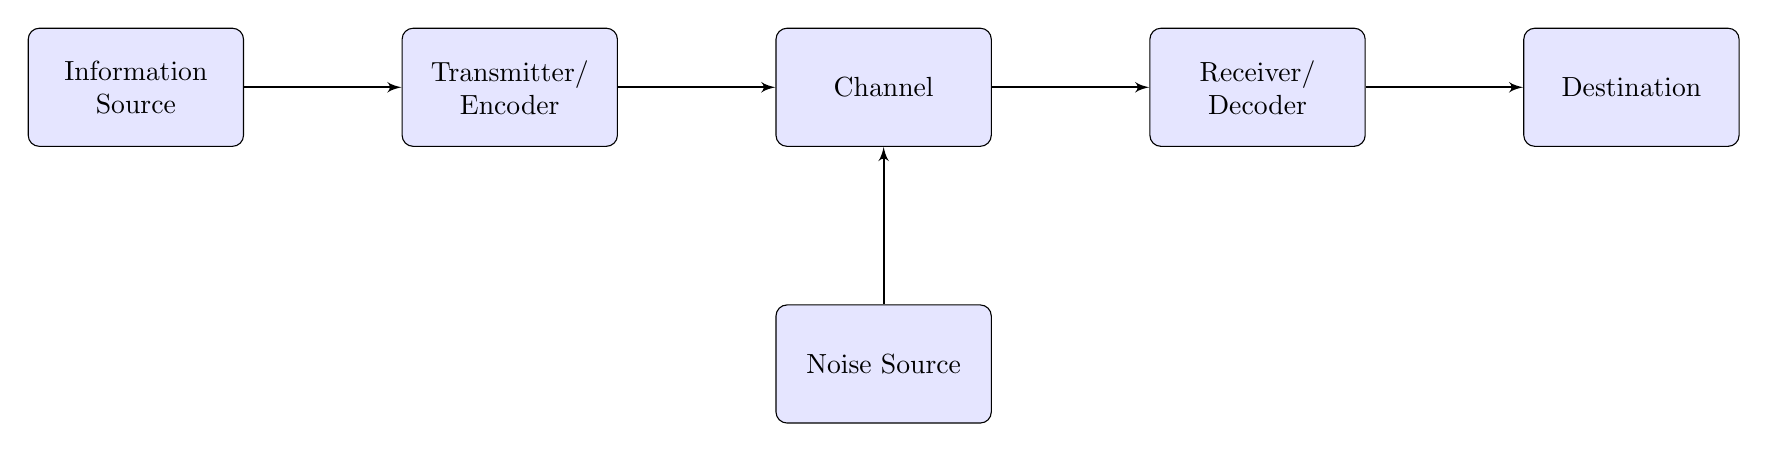
\begin{tikzpicture}[node distance=2cm, auto,
    block/.style={rectangle, draw, fill=blue!10, text width=2.5cm, text centered, rounded corners, minimum height=1.5cm},
    line/.style={draw, -latex', thick}]

    % Nodes
    \node [block] (source) {Information Source};
    \node [block, right=of source] (encoder) {Transmitter/ Encoder};
    \node [block, right=of encoder] (channel) {Channel};
    \node [block, right=of channel] (decoder) {Receiver/ Decoder};
    \node [block, right=of decoder] (dest) {Destination};
    \node [block, below=of channel] (noise) {Noise Source};

    % Paths
    \path [line] (source) -- (encoder);
    \path [line] (encoder) -- (channel);
    \path [line] (channel) -- (decoder);
    \path [line] (decoder) -- (dest);
    \path [line] (noise) -- (channel);

\end{tikzpicture}
\end{center}

\begin{itemize}
\tightlist
\end{solutionbox}
\item
  \textbf{Information Source}: Creates and decides what message to send
\item
  \textbf{Encoder/Transmitter}: Converts message into signals or code
\item
  \textbf{Channel}: Medium through which message travels
\item
  \textbf{Decoder/Receiver}: Converts signals back into understandable
  message
\item
  \textbf{Destination}: Person receiving and interpreting the message
\item
  \textbf{Noise}: Interference that disrupts clear transmission
\end{itemize}

Originally designed for technical communication, this model applies to
all forms of human interaction, showing communication as a linear
process subject to external interference.

\textbf{Mnemonic:} ``Source Encodes, Channel Carries, Destination
Decodes''

\subsubsection{2. Facial expressions and Eye
contact}\label{facial-expressions-and-eye-contact}

\begin{solutionbox}
\textbf{Answer}: Facial expressions and eye contact are powerful forms
of non-verbal communication that often convey emotions more
authentically than words.

\textbf{Table: Key Aspects of Facial Expressions and Eye Contact}

{\def\LTcaptype{none} % do not increment counter
\begin{longtable}[]{@{}
  >{\raggedright\arraybackslash}p{(\linewidth - 4\tabcolsep) * \real{0.1860}}
  >{\raggedright\arraybackslash}p{(\linewidth - 4\tabcolsep) * \real{0.2326}}
  >{\raggedright\arraybackslash}p{(\linewidth - 4\tabcolsep) * \real{0.5814}}@{}}
\toprule\noalign{}
\begin{minipage}[b]{\linewidth}\raggedright
Aspect
\end{minipage} & \begin{minipage}[b]{\linewidth}\raggedright
Function
\end{minipage} & \begin{minipage}[b]{\linewidth}\raggedright
Cultural Considerations
\end{minipage} \\
\midrule\noalign{}
\endhead
\bottomrule\noalign{}
\endlastfoot
Facial Expressions & Convey emotions (happiness, sadness, anger,
surprise) & Some expressions universal, others culture-specific \\
Eye Contact & Shows attention, confidence, interest & Duration and
intensity vary by culture \\
Micro-expressions & Brief, involuntary expressions revealing true
feelings & Often last less than 1/25 of a second \\
Eye Movement & Direction of gaze indicates thinking patterns &
Left/right movements connect to brain activity \\
\end{longtable}
}

These non-verbal cues provide critical context to verbal messages, often
revealing true feelings when words might be deceptive. Research shows
facial expressions constitute about 55\% of the emotional impact in
face-to-face communication.

\textbf{Mnemonic:} ``Face Shows What Words Can't Tell''

\end{solutionbox}
\subsection{Question 4(b) {[}4 marks{]}}\label{question-4b-4-marks}

\textbf{Choose the correct option: (Any Four)}

\begin{enumerate}
\def\labelenumi{\arabic{enumi}.}
\item
\begin{solutionbox}
  The \_\_\_ visited the stream regularly. \textbf{Answer}: C. forktail
\end{solutionbox}
\item
  Bob and Jimmy were raised in \_\_\_\_\_ just like two brothers,
\begin{solutionbox}
  together. \textbf{Answer}: B. New York
\end{solutionbox}
\item
\begin{solutionbox}
  The poet described the woods as \_\_\_\_\_\_\_. \textbf{Answer}: A.
  `lovely, dark and deep'
\end{solutionbox}
\item
\begin{solutionbox}
  Reason is compared to a clear \_\_\_\_ by Tagore. \textbf{Answer}: A.
  stream
\end{solutionbox}
\item
\begin{solutionbox}
  According to Tagore, human should work towards \_\_ \textbf{Answer}:
  B. perfection
\end{solutionbox}
\end{enumerate}

\subsection{Question 4(c) {[}7 marks{]}}\label{question-4c-7-marks}

\textbf{Write short notes: (Any Two)}

\subsubsection{1. The poet's dilemma and decision in `Stopping by Woods
on a Snowy
Evening'}\label{the-poets-dilemma-and-decision-in-stopping-by-woods-on-a-snowy-evening}

\begin{solutionbox}
\textbf{Answer}: In Robert Frost's poem, the speaker faces a momentary
conflict between pausing to appreciate natural beauty and fulfilling
responsibilities.

\textbf{Table: The Poet's Dilemma}

{\def\LTcaptype{none} % do not increment counter
\begin{longtable}[]{@{}
  >{\raggedright\arraybackslash}p{(\linewidth - 4\tabcolsep) * \real{0.3636}}
  >{\raggedright\arraybackslash}p{(\linewidth - 4\tabcolsep) * \real{0.3636}}
  >{\raggedright\arraybackslash}p{(\linewidth - 4\tabcolsep) * \real{0.2727}}@{}}
\toprule\noalign{}
\begin{minipage}[b]{\linewidth}\raggedright
Dilemma Aspect
\end{minipage} & \begin{minipage}[b]{\linewidth}\raggedright
Represented By
\end{minipage} & \begin{minipage}[b]{\linewidth}\raggedright
Resolution
\end{minipage} \\
\midrule\noalign{}
\endhead
\bottomrule\noalign{}
\endlastfoot
Attraction to Beauty & ``Lovely, dark and deep'' woods & Temporary
enjoyment \\
Practical Reality & Horse's impatience, shaking bells &
Acknowledgment \\
Social Obligations & ``Promises to keep'' & Takes precedence \\
Inner Conflict & Repeated ``miles to go before I sleep'' & Decision to
continue journey \\
\end{longtable}
}

The poet is drawn to the tranquil beauty of the snow-filled woods but
recognizes that life's responsibilities cannot be ignored indefinitely.
This represents the universal human dilemma between appreciating life's
moments of beauty and fulfilling obligations.

The decision to move on, indicated by ``miles to go before I sleep,''
shows the poet choosing duty over momentary pleasure, though the
repetition of this line suggests a lingering reluctance.

\textbf{Mnemonic:} ``Beauty Beckons, Duty Calls, Journey Continues''

\subsubsection{2. The concept of `heaven' as
expressed}\label{the-concept-of-heaven-as-expressed}

\end{solutionbox}
\begin{solutionbox}
\textbf{Answer}: In ``Where the Mind is Without Fear,'' Tagore envisions
his ideal ``heaven of freedom'' not as an afterlife destination but as a
transformed nation.

\textbf{Table: Attributes of Tagore's ``Heaven of Freedom''}

{\def\LTcaptype{none} % do not increment counter
\begin{longtable}[]{@{}
  >{\raggedright\arraybackslash}p{(\linewidth - 4\tabcolsep) * \real{0.3902}}
  >{\raggedright\arraybackslash}p{(\linewidth - 4\tabcolsep) * \real{0.3902}}
  >{\raggedright\arraybackslash}p{(\linewidth - 4\tabcolsep) * \real{0.2195}}@{}}
\toprule\noalign{}
\begin{minipage}[b]{\linewidth}\raggedright
Characteristic
\end{minipage} & \begin{minipage}[b]{\linewidth}\raggedright
Line from Poem
\end{minipage} & \begin{minipage}[b]{\linewidth}\raggedright
Meaning
\end{minipage} \\
\midrule\noalign{}
\endhead
\bottomrule\noalign{}
\endlastfoot
Fearless Thinking & ``Where the mind is without fear'' & Intellectual
freedom \\
Dignity & ``Head is held high'' & Self-respect, pride \\
Knowledge Access & ``Knowledge is free'' & Education for all, regardless
of status \\
No Divisions & ``Not broken up by narrow domestic walls'' & Unity beyond
caste, religion, region \\
Truth-Seeking & ``Words come out from the depth of truth'' & Honesty,
integrity in expression \\
Rational Thought & ``Clear stream of reason'' & Logic over
superstition \\
Purposeful Action & ``Tireless striving stretches its arms'' &
Progressive action, hard work \\
Perfection-Seeking & ``Into that heaven of freedom'' & Continuous
self-improvement \\
\end{longtable}
}

Tagore's concept represents a socio-political ideal where citizens live
with dignity and purpose, guided by reason rather than fear or
prejudice. This ``heaven'' is attainable on earth through collective
enlightenment and societal reform.

\textbf{Mnemonic:} ``Freedom, Unity, Reason, Truth, Perfection''

\subsubsection{3. The key message of `The
Leopard'}\label{the-key-message-of-the-leopard}

\end{solutionbox}
\begin{solutionbox}
\textbf{Answer}: Ruskin Bond's ``The Leopard'' conveys powerful messages
about human-nature relationships and coexistence.

\textbf{Table: Key Messages in ``The Leopard''}

{\def\LTcaptype{none} % do not increment counter
\begin{longtable}[]{@{}
  >{\raggedright\arraybackslash}p{(\linewidth - 4\tabcolsep) * \real{0.2195}}
  >{\raggedright\arraybackslash}p{(\linewidth - 4\tabcolsep) * \real{0.4634}}
  >{\raggedright\arraybackslash}p{(\linewidth - 4\tabcolsep) * \real{0.3171}}@{}}
\toprule\noalign{}
\begin{minipage}[b]{\linewidth}\raggedright
Message
\end{minipage} & \begin{minipage}[b]{\linewidth}\raggedright
Evidence in Story
\end{minipage} & \begin{minipage}[b]{\linewidth}\raggedright
Significance
\end{minipage} \\
\midrule\noalign{}
\endhead
\bottomrule\noalign{}
\endlastfoot
Mutual Respect & Leopard and author's peaceful encounters & Coexistence
is possible \\
Environmental Conservation & Author's criticism of hunters & Protection
of wildlife \\
Patience \& Observation & Author's quiet study of animals &
Understanding nature requires time \\
Human Impact & Shikaris threatening wildlife & Human activity endangers
nature \\
Nature's Beauty & Detailed descriptions of ravine ecosystem &
Appreciating wilderness \\
\end{longtable}
}

The story advocates for a deeper connection with nature through careful
observation rather than domination or exploitation. It suggests that
wild animals deserve respect and protection, not fear or hunting.

The leopard symbolizes both the majesty and vulnerability of nature,
while the author represents the potential for humans to appreciate
wildlife without harming it. This message of conservation and
coexistence remains relevant today amid environmental challenges.

\textbf{Mnemonic:} ``Respect Nature, Protect Wildlife, Observe
Patiently''

\end{solutionbox}
\subsection{OR}\label{or-3}

\subsection{Question 4(a) {[}3 marks{]}}\label{question-4a-3-marks-1}

\textbf{Write a short note: (Any One)}

\subsubsection{1. Need and Application of communication
skills}\label{need-and-application-of-communication-skills}

\begin{solutionbox}
\textbf{Answer}: Communication skills are essential abilities needed to
effectively exchange information and connect with others.

\textbf{Table: Need and Applications of Communication Skills}

{\def\LTcaptype{none} % do not increment counter
\begin{longtable}[]{@{}
  >{\raggedright\arraybackslash}p{(\linewidth - 4\tabcolsep) * \real{0.3214}}
  >{\raggedright\arraybackslash}p{(\linewidth - 4\tabcolsep) * \real{0.2143}}
  >{\raggedright\arraybackslash}p{(\linewidth - 4\tabcolsep) * \real{0.4643}}@{}}
\toprule\noalign{}
\begin{minipage}[b]{\linewidth}\raggedright
Context
\end{minipage} & \begin{minipage}[b]{\linewidth}\raggedright
Need
\end{minipage} & \begin{minipage}[b]{\linewidth}\raggedright
Applications
\end{minipage} \\
\midrule\noalign{}
\endhead
\bottomrule\noalign{}
\endlastfoot
Professional & Career advancement, leadership & Presentations,
negotiations, teamwork \\
Personal & Building relationships & Conflict resolution, emotional
support \\
Academic & Knowledge transfer & Discussions, presentations, research \\
Digital & Remote collaboration & Emails, video calls, social media \\
\end{longtable}
}

\begin{itemize}
\tightlist
\end{solutionbox}
\item
  \textbf{Workplace Applications}: Clear communication prevents errors,
  enhances productivity, improves client relationships, and facilitates
  effective leadership.
\item
  \textbf{Educational Settings}: Students with strong communication
  skills perform better in discussions, group work, and presentations.
\item
  \textbf{Personal Life}: Effective communication prevents
  misunderstandings, strengthens relationships, and helps navigate
  conflicts.
\item
  \textbf{Global Context}: Cross-cultural communication skills are
  increasingly vital in our interconnected world.
\end{itemize}

Developing these skills involves active listening, clarity in
expression, non-verbal awareness, adaptability to different contexts,
and emotional intelligence.

\textbf{Mnemonic:} ``Connect, Express, Adapt, Lead''

\subsubsection{2. Barriers to
communication}\label{barriers-to-communication}

\begin{solutionbox}
\textbf{Answer}: Communication barriers are obstacles that prevent
messages from being properly understood, creating gaps between sender
and receiver.

\textbf{Table: Major Types of Communication Barriers}

{\def\LTcaptype{none} % do not increment counter
\begin{longtable}[]{@{}
  >{\raggedright\arraybackslash}p{(\linewidth - 4\tabcolsep) * \real{0.4000}}
  >{\raggedright\arraybackslash}p{(\linewidth - 4\tabcolsep) * \real{0.2857}}
  >{\raggedright\arraybackslash}p{(\linewidth - 4\tabcolsep) * \real{0.3143}}@{}}
\toprule\noalign{}
\begin{minipage}[b]{\linewidth}\raggedright
Barrier Type
\end{minipage} & \begin{minipage}[b]{\linewidth}\raggedright
Examples
\end{minipage} & \begin{minipage}[b]{\linewidth}\raggedright
Solutions
\end{minipage} \\
\midrule\noalign{}
\endhead
\bottomrule\noalign{}
\endlastfoot
Physical & Noise, distance, technical failures & Improve environment,
use appropriate channels \\
Psychological & Bias, preconceptions, emotions & Active listening,
empathy, self-awareness \\
Semantic & Jargon, language differences & Simplify language, confirm
understanding \\
Organizational & Hierarchy, complex structures & Clear communication
channels, feedback systems \\
Cultural & Different values, customs & Cultural sensitivity,
adaptation \\
\end{longtable}
}

\begin{itemize}
\tightlist
\end{solutionbox}
\item
  \textbf{Physical Barriers}: Environmental factors that interfere with
  transmission (background noise, poor connectivity)
\item
  \textbf{Psychological Barriers}: Mental factors affecting reception
  (stress, biases, different perceptions)
\item
  \textbf{Semantic Barriers}: Problems with meaning (ambiguous words,
  technical terminology)
\item
  \textbf{Organizational Barriers}: Workplace issues (unclear roles,
  information overload)
\item
  \textbf{Cultural Barriers}: Different norms and expectations
  (gestures, etiquette, values)
\end{itemize}

Overcoming these barriers requires awareness, adaptability, feedback
mechanisms, and continuous improvement of communication practices.

\textbf{Mnemonic:} ``PPSOC: Physical, Psychological, Semantic,
Organizational, Cultural''

\subsection{Question 4(b) {[}4 marks{]}}\label{question-4b-4-marks-1}

\textbf{Choose the correct option: (Any Four)}

\begin{enumerate}
\def\labelenumi{\arabic{enumi}.}
\item
  The author clapped his hands when he saw the leopard for the first
\begin{solutionbox}
  time, because \_\_\_\_\_. \textbf{Answer}: D. he wanted to give some
  courage to himself
\end{solutionbox}
\item
  Bob and Jimmy had their last dinner together at a restaurant named
\begin{solutionbox}
  \_\_. \textbf{Answer}: D. Big Joe Brady's
\end{solutionbox}
\item
\begin{solutionbox}
  The owner of woods lives in the \_\_\_\_\_. \textbf{Answer}: C.
  village
\end{solutionbox}
\item
\begin{solutionbox}
  The woods are covered with \_\_\_. \textbf{Answer}: A. snow
\end{solutionbox}
\item
  The poem `Where the Mind is Without Fear' ends with the line:
\begin{solutionbox}
  ``\ldots let my country \_\_\_``. \textbf{Answer}: B. awake
\end{solutionbox}
\end{enumerate}

\subsection{Question 4(c) {[}7 marks{]}}\label{question-4c-7-marks-1}

\textbf{Write short notes: (Any Two)}

\subsubsection{1. The author's pain and concern in `The
Leopard'}\label{the-authors-pain-and-concern-in-the-leopard}

\begin{solutionbox}
\textbf{Answer}: In ``The Leopard,'' Ruskin Bond expresses deep
emotional distress and environmental concern regarding human impacts on
wildlife.

\textbf{Table: Author's Pain and Concern}

{\def\LTcaptype{none} % do not increment counter
\begin{longtable}[]{@{}
  >{\raggedright\arraybackslash}p{(\linewidth - 4\tabcolsep) * \real{0.2222}}
  >{\raggedright\arraybackslash}p{(\linewidth - 4\tabcolsep) * \real{0.4167}}
  >{\raggedright\arraybackslash}p{(\linewidth - 4\tabcolsep) * \real{0.3611}}@{}}
\toprule\noalign{}
\begin{minipage}[b]{\linewidth}\raggedright
Aspect
\end{minipage} & \begin{minipage}[b]{\linewidth}\raggedright
Manifestation
\end{minipage} & \begin{minipage}[b]{\linewidth}\raggedright
Significance
\end{minipage} \\
\midrule\noalign{}
\endhead
\bottomrule\noalign{}
\endlastfoot
Hunter Threat & Author's anxiety about shikaris & Direct threat to
leopard's survival \\
Habitat Destruction & Descriptions of changing landscape & Loss of
natural ecosystem \\
Human Encroachment & Increased human presence near ravine & Disruption
of animal habitats \\
Endangered Wildlife & Special focus on the leopard's vulnerability &
Symbol of threatened nature \\
Environmental Ethics & Criticism of hunting practices & Moral
questioning of human actions \\
\end{longtable}
}

The author's pain stems from witnessing the gradual destruction of a
natural paradise and the threat to creatures he has come to respect. His
particular concern for the leopard represents broader anxiety about
humanity's relationship with nature.

The emotional tone shifts from appreciation of beauty to fear for its
survival, creating a powerful environmental message. This concern
resonates today amid accelerating habitat loss and species extinction.

\textbf{Mnemonic:} ``Witness, Worry, Warn about Wildlife Threats''

\subsubsection{2. Friendship Vs. Duty in `After Twenty
Years'}\label{friendship-vs.-duty-in-after-twenty-years}

\end{solutionbox}
\begin{solutionbox}
\textbf{Answer}: O. Henry's ``After Twenty Years'' presents a powerful
moral conflict between personal loyalty and professional obligation.

\textbf{Table: Friendship vs.~Duty Conflict}

{\def\LTcaptype{none} % do not increment counter
\begin{longtable}[]{@{}
  >{\raggedright\arraybackslash}p{(\linewidth - 4\tabcolsep) * \real{0.2286}}
  >{\raggedright\arraybackslash}p{(\linewidth - 4\tabcolsep) * \real{0.4571}}
  >{\raggedright\arraybackslash}p{(\linewidth - 4\tabcolsep) * \real{0.3143}}@{}}
\toprule\noalign{}
\begin{minipage}[b]{\linewidth}\raggedright
Aspect
\end{minipage} & \begin{minipage}[b]{\linewidth}\raggedright
Friendship Side
\end{minipage} & \begin{minipage}[b]{\linewidth}\raggedright
Duty Side
\end{minipage} \\
\midrule\noalign{}
\endhead
\bottomrule\noalign{}
\endlastfoot
Bob's Perspective & Traveled miles to keep twenty-year promise & Unaware
of moral dilemma \\
Jimmy's Perspective & Values old friendship, can't face arrest &
Policeman obligated to uphold law \\
Resolution & Note explains situation, personal touch & Another officer
makes the arrest \\
Symbolic Meaning & Past bonds, personal loyalty & Present
responsibilities, social order \\
Narrative Impact & Creates story's emotional depth & Drives the ironic
twist \\
\end{longtable}
}

The story presents no easy resolution to this ethical dilemma. Jimmy
finds a compromise by arranging for another officer to make the arrest
while explaining his actions in a note, showing respect for both
friendship and duty.

O. Henry uses this conflict to explore how life choices can transform
relationships and create impossible situations where personal and
professional values collide. The story resonates because this tension
between individual connections and societal responsibilities is
universally experienced.

\textbf{Mnemonic:} ``Promises from Past, Present Principles Prevail''

\subsubsection{3. The central idea of `Stopping by Woods on a Snowy
Evening'}\label{the-central-idea-of-stopping-by-woods-on-a-snowy-evening}

\end{solutionbox}
\begin{solutionbox}
\textbf{Answer}: Robert Frost's poem explores the tension between
momentary appreciation of beauty and ongoing life responsibilities.

\textbf{Table: Central Ideas in the Poem}

{\def\LTcaptype{none} % do not increment counter
\begin{longtable}[]{@{}
  >{\raggedright\arraybackslash}p{(\linewidth - 4\tabcolsep) * \real{0.2121}}
  >{\raggedright\arraybackslash}p{(\linewidth - 4\tabcolsep) * \real{0.3030}}
  >{\raggedright\arraybackslash}p{(\linewidth - 4\tabcolsep) * \real{0.4848}}@{}}
\toprule\noalign{}
\begin{minipage}[b]{\linewidth}\raggedright
Theme
\end{minipage} & \begin{minipage}[b]{\linewidth}\raggedright
Evidence
\end{minipage} & \begin{minipage}[b]{\linewidth}\raggedright
Deeper Meaning
\end{minipage} \\
\midrule\noalign{}
\endhead
\bottomrule\noalign{}
\endlastfoot
Natural Beauty & ``Woods fill up with snow,'' ``lovely, dark and deep''
& Attraction to tranquility and wilderness \\
Responsibilities & ``Promises to keep,'' ``miles to go'' & Life's
ongoing obligations \\
Momentary Pause & Stopping between ``woods and frozen lake'' & Brief
respite from life's journey \\
Inner Conflict & Horse's questioning bell shake & Tension between desire
and duty \\
Life Journey & Repeated ``miles to go before I sleep'' & Continuing path
through life toward death \\
\end{longtable}
}

The central idea revolves around life's brief moments of contemplation
amid constant movement toward obligations. The speaker pauses to
appreciate beauty but acknowledges the impossibility of remaining in
that moment indefinitely.

The repetition of ``miles to go before I sleep'' carries dual meaning -
both the literal journey ahead and the figurative ``sleep'' of death,
suggesting the continuation of life's responsibilities until the end.
This creates a meditation on mortality, duty, and the fleeting nature of
experience.

\textbf{Mnemonic:} ``Pause, Ponder, Proceed with Purpose''

\end{solutionbox}
\subsection{Question 5(a) {[}3 marks{]}}\label{question-5a-3-marks}

\textbf{Choose the correct option: (Any Three)}

\begin{enumerate}
\def\labelenumi{\arabic{enumi}.}
\item
  If a person wants to know about various products and schemes offered
  by a merchant/company, he/she needs to write a/an \_\_\_\_\_.
\begin{solutionbox}
  \textbf{Answer}: B. Inquiry email
\end{solutionbox}
\item
  \_\_\_\_\_ indicates other persons receiving the same mail with
\begin{solutionbox}
  visible IDs. \textbf{Answer}: A. CC
\end{solutionbox}
\item
\begin{solutionbox}
  Catalogue is attached with \_\_\_\_\_. \textbf{Answer}: C. Reply to
  inquiry email
\end{solutionbox}
\item
  In which part of a formal letter/email are the key point written?
\begin{solutionbox}
  \_\_\_ \textbf{Answer}: B. Body
\end{solutionbox}
\end{enumerate}

\subsection{Question 5(b) {[}4 marks{]}}\label{question-5b-4-marks}

\textbf{Do as directed: (Any One)}

\subsubsection{1. How would you explain the terms `courtesy' and
`completeness' a
letter/email?}\label{how-would-you-explain-the-terms-courtesy-and-completeness-a-letteremail}

\begin{solutionbox}
\textbf{Answer}: Courtesy and completeness are two essential principles
of effective business communication.

\textbf{Table: Courtesy and Completeness in Business Communication}

{\def\LTcaptype{none} % do not increment counter
\begin{longtable}[]{@{}
  >{\raggedright\arraybackslash}p{(\linewidth - 4\tabcolsep) * \real{0.2821}}
  >{\raggedright\arraybackslash}p{(\linewidth - 4\tabcolsep) * \real{0.3077}}
  >{\raggedright\arraybackslash}p{(\linewidth - 4\tabcolsep) * \real{0.4103}}@{}}
\toprule\noalign{}
\begin{minipage}[b]{\linewidth}\raggedright
Principle
\end{minipage} & \begin{minipage}[b]{\linewidth}\raggedright
Definition
\end{minipage} & \begin{minipage}[b]{\linewidth}\raggedright
Implementation
\end{minipage} \\
\midrule\noalign{}
\endhead
\bottomrule\noalign{}
\endlastfoot
Courtesy & Respectful and considerate tone & Polite language, thoughtful
phrasing \\
Completeness & Including all necessary information & Answering all
questions, providing context \\
\end{longtable}
}

\textbf{Courtesy} involves treating the recipient with respect and
consideration. It manifests through:

\begin{itemize}
\tightlist
\end{solutionbox}
\item
  Using polite language (``please,'' ``thank you,'' ``kindly'')
\item
  Addressing the recipient appropriately
\item
  Avoiding demanding or accusatory tone
\item
  Showing appreciation for the recipient's time or assistance
\item
  Maintaining a positive attitude even in negative situations
\end{itemize}

\textbf{Completeness} ensures that the communication contains all
necessary information. It requires:

\begin{itemize}
\tightlist
\item
  Answering all questions or addressing all points raised
\item
  Including all relevant details (who, what, when, where, why, how)
\item
  Providing necessary background information
\item
  Anticipating potential questions and addressing them proactively
\item
  Including appropriate supporting documents or references
\end{itemize}

Both principles work together to create effective communication that
builds positive relationships while ensuring practical needs are met.

\textbf{Mnemonic:} ``Respect Fully, Inform Fully''

\subsubsection{2. Draft an application to your HOD requesting him to
grant your medical leave for two
weeks.}\label{draft-an-application-to-your-hod-requesting-him-to-grant-your-medical-leave-for-two-weeks.}

\begin{solutionbox}
\textbf{Answer}:

\begin{verbatim}
[Your Name]
[Your Class]
[Your Roll Number]
[Your College Name]
[Date]

The Head of Department
Department of [Your Department]
[College Name]
[City]

Subject: Application for Two Weeks Medical Leave

Respected Sir/Madam,

I am writing to request two weeks of medical leave from [start date] to [end date] due to [brief mention of medical condition]. I have been advised complete rest and medication by Dr. [Doctor's Name] from [Hospital/Clinic Name].

I have attached the medical certificate and prescription for your reference. During my absence, I have arranged with my classmates [Friend's Name] to share notes and assignments with me. I assure you that I will complete all pending work promptly upon my return.

I kindly request you to grant me medical leave for the mentioned period and consider this application favorably.

Thank you for your understanding and support.

Yours sincerely,

[Your Signature]
[Your Name]
[Your Roll Number]

Enclosures:
1. Medical Certificate
2. Doctor's Prescription
\end{verbatim}

\end{solutionbox}
\subsection{Question 5(c) {[}7 marks{]}}\label{question-5c-7-marks}

\textbf{Draft a letter: (Any One)}

\subsubsection{1. You are the Purchase Manager at Ashok Industries,
Sanand. Draft a letter to SP Industries, Mumbai, placing an order for 10
pieces of 9 feet lathe machines, asking for the discount
also.}\label{you-are-the-purchase-manager-at-ashok-industries-sanand.-draft-a-letter-to-sp-industries-mumbai-placing-an-order-for-10-pieces-of-9-feet-lathe-machines-asking-for-the-discount-also.}

\begin{solutionbox}
\textbf{Answer}:

\begin{verbatim}
ASHOK INDUSTRIES
Industrial Area, Phase II
Sanand - 382110, Gujarat
Tel: 02717-XXXXXX | Email: purchase@ashokind.com

January 2, 2025

The Sales Manager
SP Industries
MIDC Industrial Area
Andheri East, Mumbai - 400093

Subject: Order for 10 Pieces of 9 Feet Lathe Machines

Dear Sir/Madam,

Reference: Your Quotation No. SPI/LM/2024-523 dated December 15, 2024

We are pleased to place an order for the following equipment for our production facility at Sanand:

Item: 9 Feet Precision Lathe Machines
Model: LM-900X
Quantity: 10 pieces
Unit Price: As per your quotation (₹X,XX,XXX per unit)
Specifications:
- Motor Power: 7.5 HP
- Spindle Speed: 50-2000 RPM
- Digital Control Panel
- Hardened Bed with Steady Rest

As we are placing a bulk order, we request you to extend a special discount of 15% on the quoted price. Being a regular customer of your company, we hope you will consider our request favorably.

Payment Terms:
- 30% advance payment with purchase order
- 70% balance upon delivery and successful installation

Delivery Requirements:
- Delivery Date: Within 30 days from the date of order confirmation
- Delivery Address: Ashok Industries, Industrial Area, Phase II, Sanand - 382110, Gujarat
- Mode of Transport: By Road Transport

Please confirm receipt of this order and send us the proforma invoice including the agreed discount at your earliest convenience.

We look forward to your prompt response and timely delivery.

Yours sincerely,

[Signature]
Purchase Manager
Ashok Industries

Enclosure: Copy of Quotation No. SPI/LM/2024-523
\end{verbatim}

\subsubsection{2. Vipul Enterprise, Vapi has received a complaint from
Riya Plastics, Rajkot regarding delay in delivery of water tanks. On
behalf of Vipul Enterprise, draft a letter of
Adjustment.}\label{vipul-enterprise-vapi-has-received-a-complaint-from-riya-plastics-rajkot-regarding-delay-in-delivery-of-water-tanks.-on-behalf-of-vipul-enterprise-draft-a-letter-of-adjustment.}

\end{solutionbox}
\begin{solutionbox}
\textbf{Answer}:

\begin{verbatim}
VIPUL ENTERPRISE
Plot No. 45, GIDC
Vapi - 396195, Gujarat
Tel: 0260-XXXXXX | Email: customercare@vipulenterprise.com

January 2, 2025

The Manager
Riya Plastics
Industrial Area, Phase III
Rajkot - 360003, Gujarat

Subject: Response to Your Complaint Regarding Delayed Delivery of Water Tanks

Reference: Your Complaint Letter No. RP/VE/2024/42 dated December 25, 2024

Dear Sir/Madam,

We sincerely apologize for the delay in delivering your order of 25 water tanks (Order No. VE/WT/24/387) which was scheduled for delivery on December 20, 2024.

After investigating the matter, we found that the delay was caused by an unexpected breakdown of our production equipment, followed by transportation challenges due to the recent highway repairs between Vapi and Rajkot. We understand that this delay has affected your business operations, and we take full responsibility for this inconvenience.

As a gesture of goodwill and to compensate for the inconvenience caused, we are pleased to offer the following adjustments:

1. The remaining water tanks will be delivered to your facility by January 5, 2025, with our premium expedited shipping at no extra cost.

2. We are offering a 10% discount on your current order, which will be adjusted in the final invoice.

3. For your next three orders, we will provide a special 5% loyalty discount.

4. Our technical team will provide a complimentary inspection and maintenance service for all tanks delivered.

We value your business and the trust you have placed in Vipul Enterprise. We have implemented additional quality control measures and improved our logistics planning to ensure such delays do not occur in the future.

Please feel free to contact me directly at 98XXXXXXXX if you have any questions or require further assistance.

We appreciate your understanding and look forward to continuing our business relationship.

Yours sincerely,

[Signature]
Customer Relations Manager
Vipul Enterprise

CC: Logistics Department
\end{verbatim}

\end{solutionbox}
\subsection{OR}\label{or-4}

\subsection{Question 5(a) {[}3 marks{]}}\label{question-5a-3-marks-1}

\textbf{Choose the correct option: (Any Three)}

\begin{enumerate}
\def\labelenumi{\arabic{enumi}.}
\item
  To add/include an important point at the end in the email/letter,
\begin{solutionbox}
  \_\_\_\_\_ is used. \textbf{Answer}: A. Post Script
\end{solutionbox}
\item
\begin{solutionbox}
  When can a buyer write a complaint email? \_\_\_\_\_. \textbf{Answer}:
  D. All of these
\end{solutionbox}
\item
\begin{solutionbox}
  Give full form of C.W.O. \_\_\_\_\_. \textbf{Answer}: A. Cash with
  order
\end{solutionbox}
\item
\begin{solutionbox}
  Which of the following is an advantage of an e-mail? \textbf{Answer}:
  D. All of these
\end{solutionbox}
\end{enumerate}

\subsection{Question 5(b) {[}4 marks{]}}\label{question-5b-4-marks-1}

\textbf{Do as directed: (Any One)}

\subsubsection{1. Summarise the terms `Inside address' and
`Complimentary
Close'.}\label{summarise-the-terms-inside-address-and-complimentary-close.}

\begin{solutionbox}
\textbf{Answer}: Inside address and complimentary close are essential
components of business letter formatting that serve specific functions.

\textbf{Table: Inside Address and Complimentary Close}

{\def\LTcaptype{none} % do not increment counter
\begin{longtable}[]{@{}
  >{\raggedright\arraybackslash}p{(\linewidth - 6\tabcolsep) * \real{0.2750}}
  >{\raggedright\arraybackslash}p{(\linewidth - 6\tabcolsep) * \real{0.2500}}
  >{\raggedright\arraybackslash}p{(\linewidth - 6\tabcolsep) * \real{0.2250}}
  >{\raggedright\arraybackslash}p{(\linewidth - 6\tabcolsep) * \real{0.2500}}@{}}
\toprule\noalign{}
\begin{minipage}[b]{\linewidth}\raggedright
Component
\end{minipage} & \begin{minipage}[b]{\linewidth}\raggedright
Position
\end{minipage} & \begin{minipage}[b]{\linewidth}\raggedright
Purpose
\end{minipage} & \begin{minipage}[b]{\linewidth}\raggedright
Examples
\end{minipage} \\
\midrule\noalign{}
\endhead
\bottomrule\noalign{}
\endlastfoot
Inside Address & Left-aligned, after sender's address \& date &
Identifies recipient & The Manager, ABC Company, City \\
Complimentary Close & Before signature, aligned with date & Formal
ending & Yours sincerely, Yours faithfully \\
\end{longtable}
}

\textbf{Inside Address} appears after the sender's address and date in a
business letter. It includes:

\begin{itemize}
\tightlist
\end{solutionbox}
\item
  Recipient's name and title (if known)
\item
  Company/organization name
\item
  Complete postal address
\item
  Positioned at the left margin
\end{itemize}

It serves to identify who will receive the letter and provides necessary
information for mailing. The format should match the envelope address
exactly.

\textbf{Complimentary Close} is the formal ending of a letter that
appears before the sender's signature. Common forms include:

\begin{itemize}
\tightlist
\item
  ``Yours sincerely'' (when recipient's name is known)
\item
  ``Yours faithfully'' (when addressing by title: ``Dear Sir/Madam'')
\item
  ``Yours truly'' (alternative formal closing)
\end{itemize}

It maintains professional tone and follows standard business etiquette.
Only the first word is capitalized, and it always ends with a comma.

\textbf{Mnemonic:} ``Address Who Receives, Close Before You Sign''

\subsubsection{2. Draft an email to the Manager of GrowRich Bank, A.G.
Road Branch, Delhi to complain about the disrespectful behavior of a
staff at the
bank.}\label{draft-an-email-to-the-manager-of-growrich-bank-a.g.-road-branch-delhi-to-complain-about-the-disrespectful-behavior-of-a-staff-at-the-bank.}

\begin{solutionbox}
\textbf{Answer}:

\begin{verbatim}
From: [Your Email]
To: manager@growrichbank-agroad.com
Subject: Complaint Regarding Staff Behavior at A.G. Road Branch

Dear Manager,

Account Number: [Your Account Number]
Visit Date: January 1, 2025
Time: Approximately 11:30 AM

I am writing to express my disappointment regarding the unprofessional behavior I experienced during my recent visit to your A.G. Road Branch on January 1, 2025.

I visited the branch to update my KYC details and inquire about a home loan. While waiting for my turn at counter number 4, the staff member (with name tag "Mr. [Name]") addressed me in a dismissive tone when I asked about the documentation requirements. When I requested clarification on certain forms, he made several condescending remarks in front of other customers, stating that "everyone knows this basic information" and visibly displaying impatience.

This treatment was not only embarrassing but also contradicts the customer service standards I have come to expect from GrowRich Bank over my eight years as a loyal customer.

I request that this matter be investigated and appropriate action be taken to ensure such incidents do not recur. I would appreciate receiving:
1. An acknowledgment of this complaint
2. Information about the steps taken to address this issue
3. Assurance that bank staff receive proper training in customer interaction

I hope this matter receives your prompt attention. I can be reached at [Your Phone Number] should you need any additional information.

Thank you for your consideration.

Sincerely,

[Your Full Name]
Account Holder
Contact: [Your Phone Number]
\end{verbatim}

\end{solutionbox}
\subsection{Question 5(c) {[}7 marks{]}}\label{question-5c-7-marks-1}

\textbf{Draft an email: (Any One)}

\subsubsection{1. An email of complaint on behalf of Suraj Sharma, who
ordered a new laptop before ten days, but has yet not received it from
the AtoZ
Electronics.}\label{an-email-of-complaint-on-behalf-of-suraj-sharma-who-ordered-a-new-laptop-before-ten-days-but-has-yet-not-received-it-from-the-atoz-electronics.}

\begin{solutionbox}
\textbf{Answer}:

\begin{verbatim}
From: suraj.sharma@email.com
To: customerservice@atozelectronics.com
Cc: manager@atozelectronics.com
Subject: Complaint: Non-delivery of Laptop - Order #AZ45678

Dear Customer Service Team,

Order Reference: #AZ45678
Order Date: December 23, 2024
Expected Delivery Date: December 30, 2024
Product: Dell XPS 15 Laptop (16GB RAM, 512GB SSD)
Payment Method: Credit Card (Paid in full: ₹87,500)

I am writing to express my concern regarding the non-delivery of my laptop ordered from your online store ten days ago.

As per your confirmation email dated December 23, 2024, the laptop was supposed to be delivered within 7 working days, which should have been by December 30, 2024. Despite the payment being processed immediately, I have not received the product, nor has there been any communication from your end regarding the delay.

This situation has caused significant inconvenience as I urgently need this laptop for my professional work. I have made several attempts to contact your customer service at 1800-XXX-XXXX, but have been unable to receive any satisfactory response or concrete information about my order status.

I request immediate attention to this matter with the following actions:
1. Expedite the delivery of my laptop within the next 48 hours
2. Provide tracking information via email and SMS
3. Offer a reasonable compensation for the delay and inconvenience caused

If I do not receive the laptop or a satisfactory response by January 5, 2025, I will be compelled to escalate this matter to the consumer forum and seek a full refund.

I look forward to your prompt resolution of this issue.

Sincerely,

Suraj Sharma
Customer ID: SS78945
Mobile: 98XXXXXXXX
Address: 45, Green Park Colony, Sector 18, Gurugram - 122001
\end{verbatim}

\subsubsection{2. An email of inquiry regarding smartboards on behalf of
Excellent Coaching Classes to Best
Technologies.}\label{an-email-of-inquiry-regarding-smartboards-on-behalf-of-excellent-coaching-classes-to-best-technologies.}

\end{solutionbox}
\begin{solutionbox}
\textbf{Answer}:

\begin{verbatim}
From: director@excellentcoaching.edu
To: sales@besttechnologies.com
Subject: Inquiry: Interactive Smartboards for Educational Institution

Dear Sales Team,

I am writing on behalf of Excellent Coaching Classes, a premier coaching institute with five branches across Gujarat specializing in engineering and medical entrance exam preparation. We are looking to upgrade our classrooms with state-of-the-art interactive smartboards to enhance our teaching methodology and student engagement.

We would appreciate if you could provide us with the following information regarding your smartboard products:

1. Available models and their technical specifications:
   - Screen sizes and resolution options
   - Touch technology (infrared, capacitive, etc.)
   - Connectivity options (HDMI, USB, wireless)
   - Software compatibility and features

2. Educational features and capabilities:
   - Pre-loaded educational software and applications
   - Content creation and sharing capabilities
   - Recording and playback functions
   - Multi-user collaboration features

3. Commercial details:
   - Pricing for different models
   - Bulk purchase discounts (we require approximately 20 boards)
   - Warranty period and terms
   - Installation services and charges
   - Annual maintenance contract options

4. Training and support:
   - Training for teaching staff
   - Technical support availability
   - Troubleshooting and maintenance procedures

Additionally, we would like to know if you offer a demonstration of your products at our main facility in Ahmedabad. If possible, we would like to schedule a demo during the coming week.

Please include your product catalog and any relevant brochures with your response. We look forward to your detailed reply at your earliest convenience.

Thank you for your assistance.

Best regards,

Dr. Rajesh Patel
Director
Excellent Coaching Classes
Address: 56, Education Hub, Navrangpura, Ahmedabad - 380009
Tel: 079-XXXXXXXX
Mobile: 98XXXXXXXX
Website: www.excellentcoaching.edu
\end{verbatim}

\end{solutionbox}
\subsection{Summary of Key Concepts}\label{summary-of-key-concepts}

{\def\LTcaptype{none} % do not increment counter
\begin{longtable}[]{@{}
  >{\raggedright\arraybackslash}p{(\linewidth - 4\tabcolsep) * \real{0.1750}}
  >{\raggedright\arraybackslash}p{(\linewidth - 4\tabcolsep) * \real{0.4500}}
  >{\raggedright\arraybackslash}p{(\linewidth - 4\tabcolsep) * \real{0.3750}}@{}}
\toprule\noalign{}
\begin{minipage}[b]{\linewidth}\raggedright
Topic
\end{minipage} & \begin{minipage}[b]{\linewidth}\raggedright
Important Points
\end{minipage} & \begin{minipage}[b]{\linewidth}\raggedright
Learning Tips
\end{minipage} \\
\midrule\noalign{}
\endhead
\bottomrule\noalign{}
\endlastfoot
Communication Models & SMCR model focuses on Sender, Message, Channel,
Receiver & Think S-M-C-R as a sequence \\
Verbal vs.~Non-verbal & Words vs.~gestures, expressions, tone;
complement each other & Notice how tone affects meaning \\
Communication Barriers & Physical, psychological, semantic,
organizational, cultural & Remember PPSOC acronym \\
Sentence Patterns & SV, SVO, SVC, SVA - basic English structures &
Identify subject and verb first \\
Modal Auxiliaries & Express ability, permission, obligation, possibility
& Connect to function (can = ability) \\
Subject-Verb Agreement & Singular subjects take singular verbs & Check
subject before choosing verb \\
Parts of Speech & Nouns, verbs, adjectives, adverbs, prepositions, etc.
& Watch word function in sentence \\
Tenses & Present, past, future in simple, continuous, perfect forms &
Focus on time and aspect \\
Business Letters & Formal structure with sender/receiver details,
subject, body & Follow standard format templates \\
Emails & Concise, clear messages with appropriate subject lines & Use
proper digital etiquette \\
Literature Analysis & Themes in poems and stories connect to human
experiences & Look for author's message and symbolism \\
\end{longtable}
}

\textbf{Study Tips for Weak Students:}

\begin{enumerate}
\def\labelenumi{\arabic{enumi}.}
\tightlist
\item
  \textbf{For grammar questions}:

  \begin{itemize}
  \tightlist
  \item
    Learn one sentence pattern per day
  \item
    Practice identifying parts of speech in simple sentences
  \item
    Make flashcards for modal auxiliaries and their functions
  \end{itemize}
\item
  \textbf{For communication concepts}:

  \begin{itemize}
  \tightlist
  \item
    Draw simple diagrams of communication models
  \item
    List examples of barriers you've experienced personally
  \item
    Create a chart comparing verbal and non-verbal communication
  \end{itemize}
\item
  \textbf{For literature}:

  \begin{itemize}
  \tightlist
  \item
    Read summaries first to understand the basic story
  \item
    Focus on main characters and their motivations
  \item
    Identify 1-2 key themes in each piece
  \end{itemize}
\item
  \textbf{For business communication}:

  \begin{itemize}
  \tightlist
  \item
    Memorize letter and email templates
  \item
    Practice writing at least one email/letter each week
  \item
    Study standard phrases used in formal communication
  \end{itemize}
\end{enumerate}

Remember: Regular practice is more effective than cramming before exams!

\end{document}